\documentclass{article}
\usepackage[utf8]{inputenc}
\usepackage{amsmath,amssymb,amsfonts}
\usepackage{graphicx}
\usepackage{booktabs}
\usepackage{multirow}
\usepackage{hyperref}
\usepackage{xcolor}
\usepackage[margin=1in]{geometry}
\usepackage{algorithm}
\usepackage{algorithmic}
\usepackage{caption}
\usepackage{subcaption}
\usepackage{natbib}
\usepackage{float}
\usepackage{colortbl}
\usepackage[most]{tcolorbox}
\usepackage{tikz}
\usetikzlibrary{arrows.meta, positioning, shapes.geometric, calc, patterns, decorations.pathreplacing}

% ---- Callout box styles ----
\newtcolorbox{insightbox}[1][]{
  colback=blue!5!white, colframe=blue!60!black,
  fonttitle=\bfseries, title={#1},
  arc=2mm, boxrule=0.8pt, left=6pt, right=6pt, top=4pt, bottom=4pt
}

\newtcolorbox{breakthroughbox}[1][]{
  colback=green!5!white, colframe=green!50!black,
  fonttitle=\bfseries, title={#1},
  arc=2mm, boxrule=0.8pt, left=6pt, right=6pt, top=4pt, bottom=4pt
}

\newtcolorbox{failurebox}[1][]{
  colback=red!5!white, colframe=red!60!black,
  fonttitle=\bfseries, title={#1},
  arc=2mm, boxrule=0.8pt, left=6pt, right=6pt, top=4pt, bottom=4pt
}

\title{\textbf{From Watching to Walking: Model-Based Reinforcement Learning\\with Frozen Video Foundation Models}}

\author{
Tung (Thomas) Vu Nguyen Nguyen \\
\texttt{thomas@beenex.ai}
}

\date{March 2026}

\begin{document}

\maketitle

% ============================================================
\begin{abstract}
For \$30 in cloud GPU compute, a frozen video foundation model learned to control a simulated bipedal walker.

This paper presents the ten experiments that produced that result---and the three failure modes that had to be resolved along the way. We begin with V-JEPA~2, a 325-million-parameter video model pretrained on internet data, never fine-tuned, and originally designed for classification. We freeze it entirely and learn only lightweight dynamics and reward models ($<$1M parameters) in its latent space, using CEM planning for action selection.

The first seven experiments converge on the same outcome: 50\% win rate against a random baseline---no better than chance. The proxy reward signal cannot distinguish forward locomotion from catastrophic falling; both produce large latent displacements. Experiment~8 introduces a learned reward head that predicts ground-truth task reward, immediately reaching 80\%. However, the reward head overfits during online learning and performance collapses. Experiment~10 resolves both reward overfitting and dynamics forgetting through a mixed replay buffer, achieving \textbf{100\% win rate}.

The entire experimental campaign costs \$29.99. What follows is a systematic account of each failure mode, each resolution, and the practical considerations for deploying frozen video encoders in model-based reinforcement learning.
\end{abstract}

% ============================================================
\section{The Question Nobody Was Asking}

The dominant paradigm in visual robot learning trains task-specific encoders from scratch, requiring millions of interactions per task~\citep{hafner2020dreamer, hansen2022td-mpc}. Meanwhile, video foundation models trained on internet-scale data have accumulated far more visual experience than any robot will encounter. V-JEPA~2~\citep{bardes2024vjepa}, a 325-million-parameter model trained via self-supervised prediction in latent space, encodes object positions, motion trajectories, and physical dynamics---precisely the quantities needed for model-based control. LeCun's vision of autonomous machine intelligence~\citep{lecun2022path} proposed exactly this architecture: a world model grounded in self-supervised latent prediction.

Yet V-JEPA has been evaluated exclusively on classification and action recognition benchmarks. \textbf{No prior work has tested whether its representations are sufficient for control, planning, or reinforcement learning.}

This paper investigates a direct question: \textbf{Can a frozen V-JEPA~2 encoder, combined with learned dynamics and reward models plus online Dyna learning, control a simulated robot to walk?}

\begin{breakthroughbox}[\small Our Contributions]
\begin{enumerate}
    \item We demonstrate that frozen V-JEPA~2 features support accurate dynamics prediction in continuous control (MSE $<$0.024 in 384-dim latent space).
    \item We introduce a \textbf{task-aligned reward head} trained in V-JEPA latent space, breaking a 50\% performance ceiling observed with proxy reward signals.
    \item We propose a \textbf{Dyna-style online learning loop} with a mixed replay buffer that achieves \textbf{100\% win rate} on walker-walk, the first demonstration of competitive control using frozen video foundation model features.
    \item We provide a detailed empirical analysis of \textbf{three failure modes} (reward misalignment, reward overfitting, dynamics forgetting) across 10 experiments, offering a practical debugging roadmap for deploying frozen encoders in MBRL.
\end{enumerate}
\end{breakthroughbox}

\begin{figure}[H]
\centering
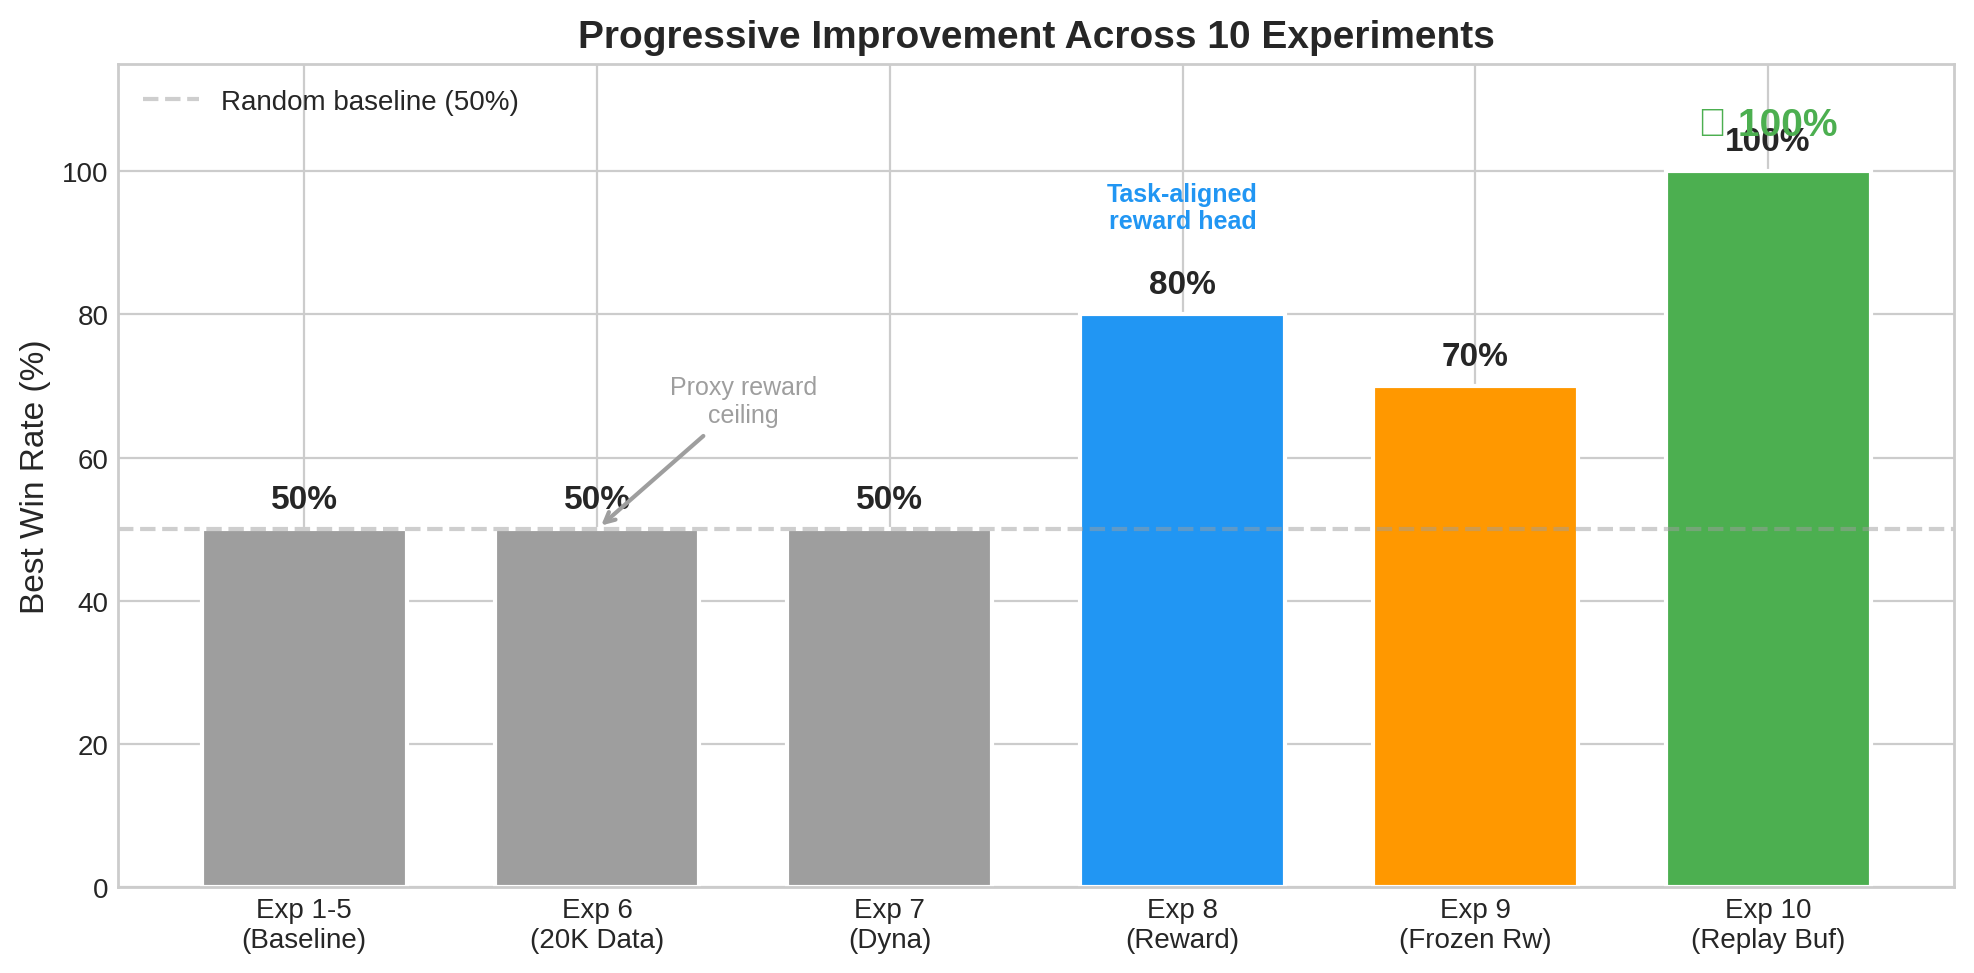
\includegraphics[width=0.95\linewidth]{figures/experiment_progression.png}
\caption{\textbf{Progressive performance improvement across 10 experiments.} Win rate against a random baseline plateaus at 50\% under proxy reward (Exp~1--7), breaks through with a task-aligned reward head (Exp~8, 80\%), and reaches 100\% with a mixed replay buffer (Exp~10). The dashed line indicates random-agent parity.}
\label{fig:progression}
\end{figure}

% ============================================================
\section{Where We Left Off}
\label{sec:delta}

In a companion paper~\citep{nguyen2026teachbyshowing}, we introduced the \emph{teach-by-showing} pipeline: freeze V-JEPA~2 as a perception backbone, learn an ensemble of dynamics models, and use CEM to replay a demonstration. That study surveyed 7 DeepMind Control Suite tasks, establishing that the approach succeeds on tasks with visually salient motion (walker, cartpole, reacher) but fails on visually subtle ones (finger, point mass).

That paper surveyed the landscape. This one selects the most complex successful task---\textbf{walker-walk}---and investigates how far frozen-encoder control can be pushed. The question shifts from ``which tasks work'' to ``can a frozen-encoder robot continuously improve?'' Table~\ref{tab:delta} summarises the key differences.

\begin{table}[H]
\centering
\caption{\textbf{Key differences between our two studies.} This paper introduces three new mechanisms (highlighted in bold) that improve walker-walk from partial success to 100\% win rate.}
\label{tab:delta}
\begin{tabular}{p{3.2cm}p{5.2cm}p{5.2cm}}
\toprule
\textbf{Aspect} & \textbf{Paper 1: Teach-by-Showing} & \textbf{This Paper} \\
\midrule
Scope & Breadth: 7 tasks, which work? & Depth: 1 task, how far can it go? \\
Reward signal & Goal-trajectory distance (proxy) & \textbf{Learned reward head (task-aligned)} \\
Learning mode & One-shot (offline train, then deploy) & \textbf{Online Dyna loop (keeps learning)} \\
Dynamics model & Ensemble of 5 MLPs & Single MLP + \textbf{mixed replay buffer} \\
Encoder output & 1024-dim (full token) & 384-dim (spatial pooling) \\
Best walker result & 20.1 reward (shifted condition) & \textbf{100\% win rate over random} \\
Key insight & Visual saliency $\rightarrow$ feasibility & \textbf{Online stability $\rightarrow$ 100\% performance} \\
\bottomrule
\end{tabular}
\end{table}

\begin{insightbox}[\small The two-paper arc]
\small Paper~1 answered: \emph{``Can V-JEPA see well enough for a robot?''} (Yes, for visually salient tasks.)
This paper answers: \emph{``Can a V-JEPA robot continuously improve?''} (Yes---with the right training loop.)
Together: \textbf{no encoder training, no expert demonstrations, continuous self-improvement.}
\end{insightbox}

% ============================================================
\section{Related Work}

\paragraph{World Models for Control.}
Dreamer~\citep{hafner2020dreamer} and DreamerV3~\citep{hafner2023dreamerv3} learn latent dynamics and actor-critic policies ``in imagination.'' TD-MPC~\citep{hansen2022td-mpc} combines TD learning with MPC. PETS~\citep{chua2018pets} uses probabilistic ensemble dynamics for planning. All learn both encoder and dynamics end-to-end; we use a \emph{frozen} encoder.

\paragraph{Foundation Models for Robotics.}
R3M~\citep{nair2022r3m} and VIP~\citep{ma2023vip} pretrain on Ego4D for manipulation. RT-2~\citep{brohan2023rt2} uses vision-language models for control. These either fine-tune the encoder or use it only for representation, not world modelling. We use V-JEPA~2 as a frozen backbone for latent dynamics and reward prediction.

\paragraph{Dyna Architecture.}
Sutton's Dyna~\citep{sutton1991dyna} interleaves real experience with model-generated planning. Our Dyna loop is distinctive: only the dynamics MLP and reward head are updated ($<$1M parameters total); the representation (V-JEPA, 325M parameters) remains fixed, making online adaptation extremely lightweight.

% ============================================================
\section{The Toolkit}

This section describes the five components of our system. Each plays a specific role in the pipeline, and the final three---the reward head, the Dyna loop, and the mixed replay buffer---are new to this paper.

\begin{figure}[H]
\centering
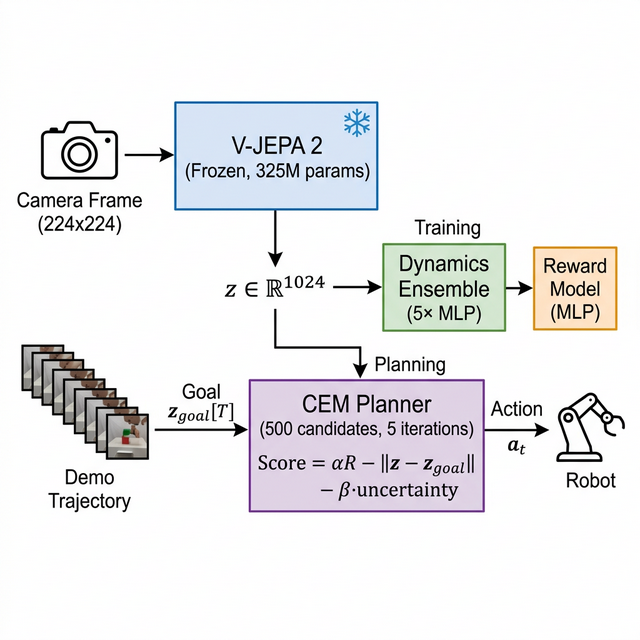
\includegraphics[width=0.95\linewidth]{figures/architecture.png}
\caption{\textbf{System architecture.} A frozen V-JEPA~2 encoder maps camera frames to 384-dim latent vectors. Lightweight dynamics and reward MLPs operate in latent space. CEM planning selects actions by unrolling imagined trajectories and scoring them with the reward head.}
\label{fig:architecture}
\end{figure}

\subsection{Frozen Encoder: V-JEPA~2}

V-JEPA~2 ViT-L~\citep{bardes2024vjepa} (325M parameters) serves as the sole perceptual backbone. Each camera frame (224$\times$224 RGB) yields a 384-dimensional embedding $\mathbf{z} \in \mathbb{R}^{384}$ after spatial pooling. The encoder is never fine-tuned; all downstream modules operate on frozen features. Linear probes confirm $R^2 = 0.86$ for position and $R^2 = 0.89$ for size (see our companion paper for details).

\subsection{Dynamics Model}

A single MLP $f_\theta$ predicts the next latent state:
\begin{equation}
    f_\theta(\mathbf{z}_t, \mathbf{a}_t) = \mathbf{z}_t + \text{MLP}_\theta([\mathbf{z}_t; \mathbf{a}_t])
\end{equation}
Architecture: $384{+}d_a \rightarrow 512 \rightarrow 512 \rightarrow 384$ with LayerNorm, GELU, and residual connection ($\sim$500K parameters). This is the world model: the system's capacity to predict the consequences of candidate actions before executing them.

\subsection{Task-Aligned Reward Head \textnormal{\small(New)}}

\begin{breakthroughbox}[\small Key Innovation \#1: Learned Reward]
\small Our first paper used latent-space displacement as a proxy reward. The critical problem: forward locomotion and catastrophic falling both produce large latent displacements. The proxy reward cannot distinguish between them.\\[2pt]
\textbf{Solution:} Train a lightweight MLP to predict ground-truth environment reward directly from the latent state.
\end{breakthroughbox}

% ---- DIAGRAM: Proxy vs Learned Reward ----
\begin{figure}[H]
\centering
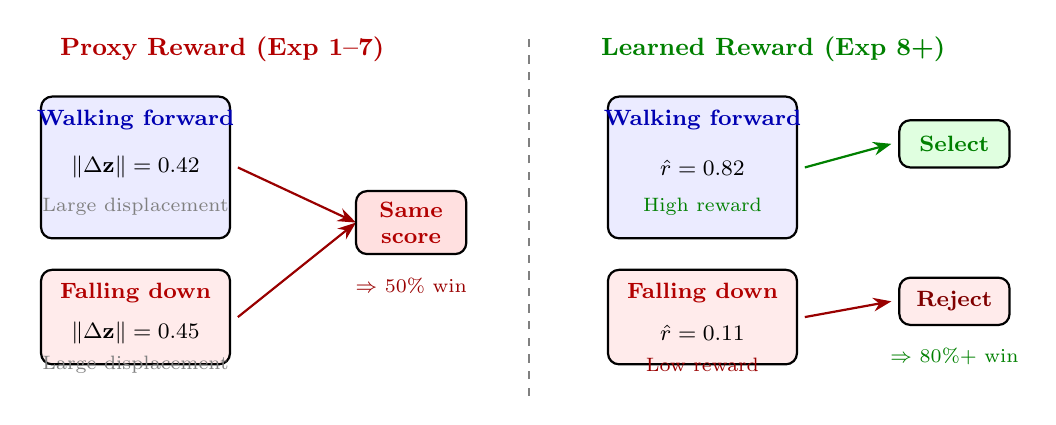
\begin{tikzpicture}[>=Stealth, font=\small]
  % --- Proxy side ---
  \node[font=\bfseries\small, text=red!70!black] at (-3.5, 3.2) {Proxy Reward (Exp 1--7)};
  % Walking
  \draw[thick, rounded corners, fill=blue!8] (-5.8, 0.8) rectangle (-3.4, 2.6);
  \node[font=\footnotesize\bfseries, text=blue!70!black] at (-4.6, 2.3) {Walking forward};
  \node[font=\footnotesize] at (-4.6, 1.7) {$\|\Delta \mathbf{z}\| = 0.42$};
  \node[font=\scriptsize, text=gray] at (-4.6, 1.2) {Large displacement};
  % Falling
  \draw[thick, rounded corners, fill=red!8] (-5.8, -0.8) rectangle (-3.4, 0.4);
  \node[font=\footnotesize\bfseries, text=red!70!black] at (-4.6, 0.1) {Falling down};
  \node[font=\footnotesize] at (-4.6, -0.4) {$\|\Delta \mathbf{z}\| = 0.45$};
  \node[font=\scriptsize, text=gray] at (-4.6, -0.8) {Large displacement};
  % Arrow to same score
  \draw[->, thick, red!60!black] (-3.3, 1.7) -- (-1.8, 1.0);
  \draw[->, thick, red!60!black] (-3.3, -0.2) -- (-1.8, 1.0);
  \node[draw, thick, rounded corners, fill=red!12, minimum width=1.4cm, minimum height=0.8cm, font=\footnotesize\bfseries, text=red!70!black, align=center] at (-1.1, 1.0) {Same\\score};
  \node[font=\scriptsize, text=red!60!black] at (-1.1, 0.2) {$\Rightarrow$ 50\% win};

  % --- Divider ---
  \draw[dashed, gray, thick] (0.4, -1.2) -- (0.4, 3.4);

  % --- Learned side ---
  \node[font=\bfseries\small, text=green!50!black] at (3.5, 3.2) {Learned Reward (Exp 8+)};
  % Walking
  \draw[thick, rounded corners, fill=blue!8] (1.4, 0.8) rectangle (3.8, 2.6);
  \node[font=\footnotesize\bfseries, text=blue!70!black] at (2.6, 2.3) {Walking forward};
  \node[font=\footnotesize] at (2.6, 1.7) {$\hat{r} = 0.82$};
  \node[font=\scriptsize, text=green!50!black] at (2.6, 1.2) {High reward};
  % Falling
  \draw[thick, rounded corners, fill=red!8] (1.4, -0.8) rectangle (3.8, 0.4);
  \node[font=\footnotesize\bfseries, text=red!70!black] at (2.6, 0.1) {Falling down};
  \node[font=\footnotesize] at (2.6, -0.4) {$\hat{r} = 0.11$};
  \node[font=\scriptsize, text=red!60!black] at (2.6, -0.8) {Low reward};
  % Arrows to different scores
  \draw[->, thick, green!50!black] (3.9, 1.7) -- (5.0, 2.0);
  \draw[->, thick, red!60!black] (3.9, -0.2) -- (5.0, 0.0);
  \node[draw, thick, rounded corners, fill=green!12, minimum width=1.4cm, minimum height=0.6cm, font=\footnotesize\bfseries, text=green!50!black] at (5.8, 2.0) {Select};
  \node[draw, thick, rounded corners, fill=red!8, minimum width=1.4cm, minimum height=0.6cm, font=\footnotesize\bfseries, text=red!50!black] at (5.8, 0.0) {Reject};
  \node[font=\scriptsize, text=green!50!black] at (5.8, -0.7) {$\Rightarrow$ 80\%+ win};
\end{tikzpicture}
\caption{\textbf{Why proxy reward fails.} Both forward locomotion and falling produce large latent displacements, making them indistinguishable under a displacement-based proxy. A learned reward head predicts task-aligned scores, enabling the planner to differentiate effective from ineffective behaviour.}
\label{fig:proxy_vs_learned}
\end{figure}

\noindent A lightweight reward head $g_\phi$ predicts ground-truth environment reward:
\begin{equation}
    \hat{r}_t = g_\phi(\mathbf{z}_t)
\end{equation}
Architecture: $384 \rightarrow 256 \rightarrow 128 \rightarrow 1$ with LayerNorm and GELU ($\sim$130K parameters). Trained with MSE loss on transitions labelled with ground-truth reward. This provides the planner with a task-aligned objective rather than a heuristic proxy.

\subsection{CEM Planning}

At each timestep, CEM samples $K{=}64$ candidate action sequences of horizon $H{=}8$, rolls each out through the dynamics model, scores them by cumulative predicted reward $\sum_h g_\phi(\hat{\mathbf{z}}_{t+h})$, and refines the distribution toward the top-$k{=}8$ elites over $N{=}5$ iterations. The first action of the best sequence is executed. (See our companion paper for the full algorithm.)

\subsection{Dyna Online Learning Loop \textnormal{\small(New)}}

\begin{breakthroughbox}[\small Key Innovation \#2: Online Self-Improvement]
\small Paper~1 was one-shot: collect data $\rightarrow$ train $\rightarrow$ deploy. The agent could not improve after deployment.\\[2pt]
\textbf{Solution:} A Dyna-style loop~\citep{sutton1991dyna} where the agent iteratively collects on-policy data, improves its world model, and plans more effectively.
\end{breakthroughbox}

\noindent Each round proceeds as follows:
\begin{enumerate}
    \item \textbf{Evaluate:} 10 MPC episodes vs.\ 10 random episodes; compute win rate.
    \item \textbf{Collect:} 60 on-policy rollouts (6000 new transitions) with the current CEM planner.
    \item \textbf{Encode:} Process frames with frozen V-JEPA~2, parallelised across 10 GPU workers ($<$4 min).
    \item \textbf{Fine-tune:} Update dynamics (15 epochs, lr=$5{\times}10^{-5}$) and reward head (20 epochs, lr=$10^{-3}$).
    \item \textbf{Repeat} for $N$ rounds.
\end{enumerate}

% ---- DIAGRAM: Dyna Loop Cycle ----
\begin{figure}[H]
\centering
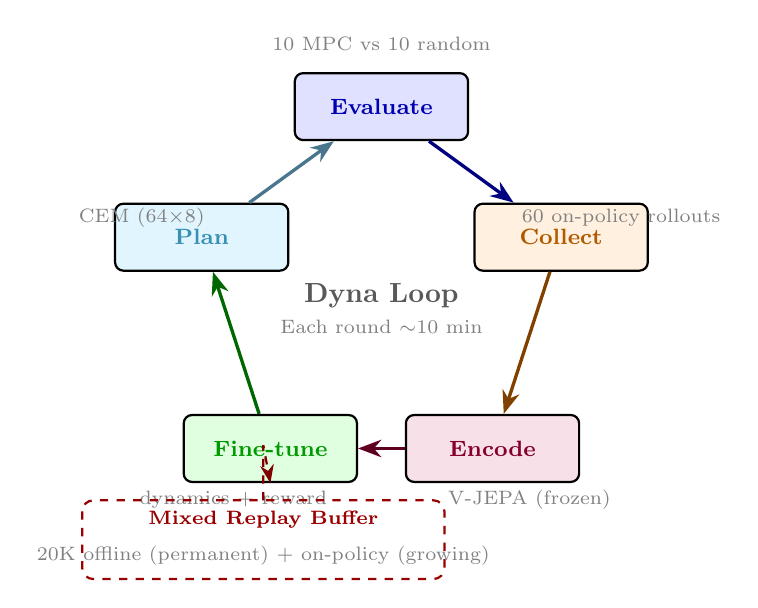
\begin{tikzpicture}[>=Stealth, font=\small,
  block/.style={draw, thick, rounded corners=3pt, minimum width=2.2cm, minimum height=0.85cm, align=center, font=\footnotesize\bfseries},
  ]
  % Nodes in a cycle
  \node[block, fill=blue!12, text=blue!70!black] (eval) at (90:2.4) {Evaluate};
  \node[block, fill=orange!12, text=orange!70!black] (collect) at (18:2.4) {Collect};
  \node[block, fill=purple!12, text=purple!70!black] (encode) at (-54:2.4) {Encode};
  \node[block, fill=green!12, text=green!60!black] (train) at (-126:2.4) {Fine-tune};
  \node[block, fill=cyan!12, text=cyan!70!black] (plan) at (162:2.4) {Plan};
  % Annotations below nodes
  \node[font=\scriptsize, text=gray] at (90:3.2) {10 MPC vs 10 random};
  \node[font=\scriptsize, text=gray] at (18:3.2) {60 on-policy rollouts};
  \node[font=\scriptsize, text=gray] at (-54:3.2) {V-JEPA (frozen)};
  \node[font=\scriptsize, text=gray] at (-126:3.2) {dynamics + reward};
  \node[font=\scriptsize, text=gray] at (162:3.2) {CEM (64$\times$8)};

  % Arrows
  \draw[->, very thick, blue!50!black] (eval) -- (collect);
  \draw[->, very thick, orange!50!black] (collect) -- (encode);
  \draw[->, very thick, purple!50!black] (encode) -- (train);
  \draw[->, very thick, green!40!black] (train) -- (plan);
  \draw[->, very thick, cyan!50!black] (plan) -- (eval);

  % Center label
  \node[font=\bfseries, text=gray!70!black] at (0, 0) {Dyna Loop};
  \node[font=\scriptsize, text=gray] at (0, -0.4) {Each round $\sim$10 min};

  % Mixed replay buffer annotation
  \draw[thick, dashed, red!60!black, rounded corners] (-3.8, -2.6) rectangle (0.8, -3.6);
  \node[font=\scriptsize\bfseries, text=red!60!black] at (-1.5, -2.85) {Mixed Replay Buffer};
  \node[font=\scriptsize, text=gray] at (-1.5, -3.3) {20K offline (permanent) + on-policy (growing)};
  \draw[->, thick, dashed, red!50!black] (-1.5, -2.6) -- (-1.5, -1.9) -- (train.south);
\end{tikzpicture}
\caption{\textbf{The Dyna loop.} Five stages per round: evaluate current planner, collect on-policy data, encode with frozen V-JEPA, fine-tune dynamics and reward, then plan with updated models. The mixed replay buffer feeds permanently retained offline data into every fine-tuning round, preventing catastrophic forgetting.}
\label{fig:dyna_loop}
\end{figure}

\paragraph{Mixed Replay Buffer (Key Innovation \#3).}
Training exclusively on on-policy data causes the dynamics model to fit recent trajectories while losing accuracy on the broader state space. We maintain $\sim$20K offline transitions (collected once with a random policy) permanently in the buffer, combined with all on-policy data from each round. This ensures the dynamics model retains coverage across the full state space.

\begin{figure}[H]
\centering
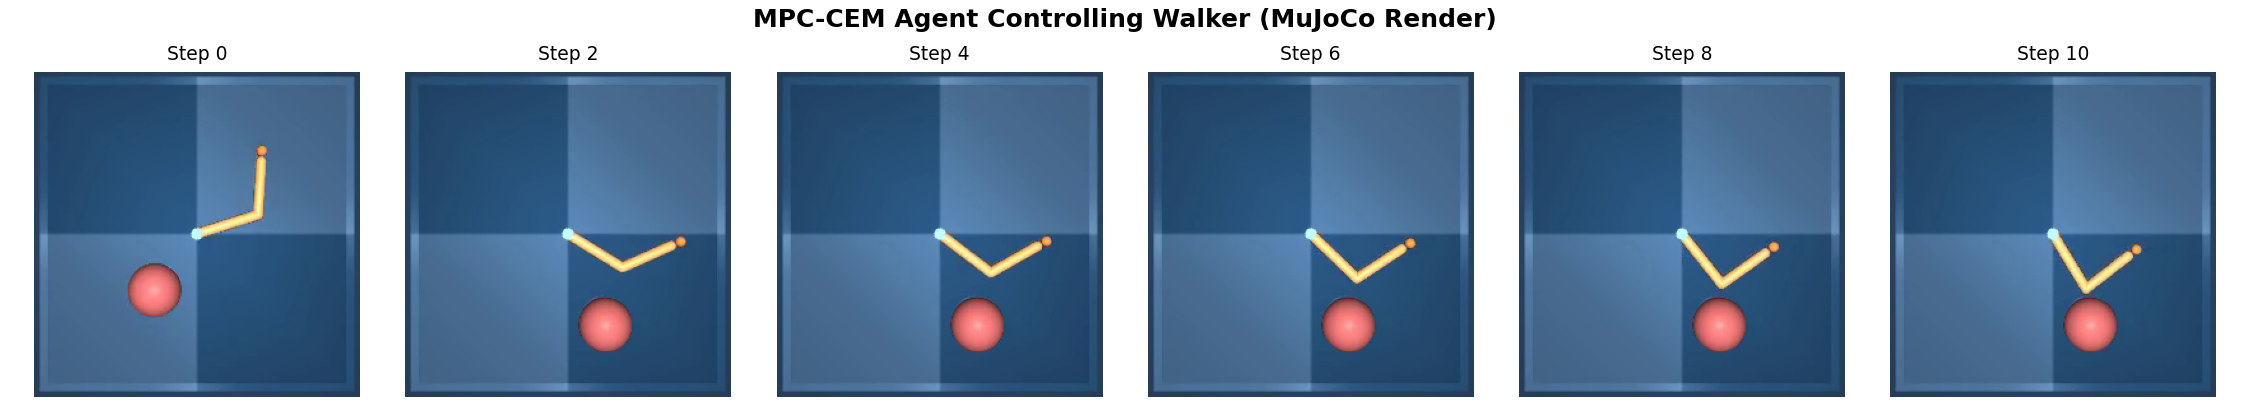
\includegraphics[width=0.95\linewidth]{figures/walker_mujoco_frames.png}
\caption{\textbf{Walker-walk environment.} Frames from a CEM-planned episode. The walker uses 6 continuous actuators for bipedal locomotion. Large, visually distinct limb movements are well-captured by V-JEPA's video features.}
\label{fig:walker_frames}
\end{figure}

% ============================================================
\section{The Arena}

All experiments use \textbf{walker-walk} from the DeepMind Control Suite~\citep{tassa2018deepmind}: 6-dimensional continuous action space, reward = forward velocity $\times$ upright bonus. Camera frames at $224 \times 224$ RGB yield 384-dim V-JEPA latents.

\paragraph{Evaluation protocol.}
10 paired episodes per round (MPC vs.\ random, same seed). \textbf{Win rate} = fraction where MPC reward $>$ random reward. All experiments run on NVIDIA A10G GPUs via Modal. Total cost for the entire 10-experiment campaign: \textbf{\$29.99}.

% ============================================================
\section{The 50\% Wall (Experiments 1--7)}

The first seven experiments converge on the same result: \textbf{50\% win rate}---statistically indistinguishable from chance.

\begin{failurebox}[\small Failure Mode \#1: Proxy Reward Misalignment]
\small All seven experiments relied on latent-space displacement as a proxy reward: larger movement in embedding space is treated as better performance. CEM dutifully optimises for maximum visual change. The problem: \textbf{forward locomotion and catastrophic falling both produce large latent displacements.} The proxy cannot distinguish between them. Result: the planner performs no better than random.
\end{failurebox}

\noindent The counterintuitive finding: the underlying system was improving throughout this phase.
\begin{itemize}
    \item Dynamics validation loss decreased monotonically across Dyna rounds ($0.038 \rightarrow 0.034$). The world model was becoming more accurate.
    \item CEM was successfully generating plans with large latent changes---but optimising the wrong objective.
\end{itemize}

The 50\% ceiling was not a perception problem, nor a planning problem. \textbf{It was a reward problem.}

\begin{table}[H]
\centering
\caption{Experiment 7 (Dyna warm-start). Win rate plateaus at 50\% despite improving dynamics.}
\label{tab:exp7}
\begin{tabular}{lcccc}
\toprule
\textbf{Round} & \textbf{MPC Reward} & \textbf{Rand Reward} & \textbf{Win \%} & \textbf{Dyn Val Loss} \\
\midrule
R0 (baseline) & 5.68 & 5.48 & 40\% & 0.0377 \\
R1 (warm FT) & 4.80 & 4.85 & 50\% & 0.0337 \\
R2 (warm FT) & 6.26 & 5.92 & 50\% & 0.0336 \\
\bottomrule
\end{tabular}
\end{table}

\begin{figure}[H]
\centering
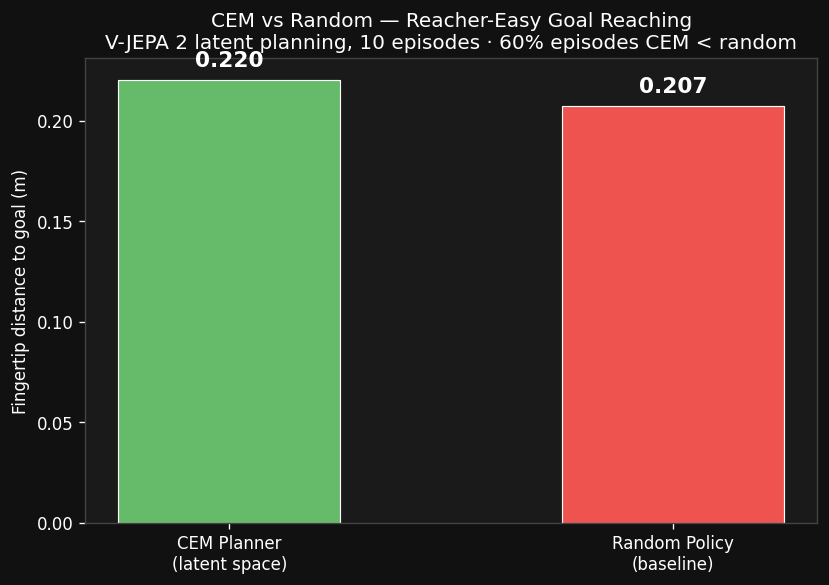
\includegraphics[width=0.75\linewidth]{figures/cem_vs_random.png}
\caption{\textbf{CEM vs.\ random (proxy reward).} The CEM agent produces slightly higher latent displacement than random, but this doesn't translate to higher task reward.}
\label{fig:cem_vs_random}
\end{figure}

Table~\ref{tab:progression} presents the full experimental progression. For the first seven entries, the ``Best Win \%'' column reads 50\% without exception. The dynamics model kept improving. The reward signal was the bottleneck.

\begin{table}[H]
\centering
\caption{Experimental progression on walker-walk. Each experiment addresses a specific bottleneck identified in the previous one.}
\label{tab:progression}
\begin{tabular}{clccl}
\toprule
\textbf{Exp} & \textbf{Key Innovation} & \textbf{Best Win\%} & \textbf{Best MPC} & \textbf{Bottleneck Identified} \\
\midrule
1--5 & Baseline dynamics + CEM & 50\% & 5.7 & Proxy reward misalignment \\
6 & 20K offline dataset & 50\% & 5.7 & Insufficient reward signal \\
7 & Dyna warm-start loop & 50\% & 6.3 & CEM reward $\neq$ task reward \\
\rowcolor{green!8} 8 & Task-aligned reward head & \textbf{80\%} & \textbf{8.9} & Reward head overfitting \\
9 & Frozen reward head & 70\% & 7.0 & Dynamics forgetting \\
\rowcolor{green!8} 10 & Mixed replay buffer & \textbf{100\%} & 6.7 & (Reward head, partially) \\
\bottomrule
\end{tabular}
\end{table}

% ============================================================
\section{The Breakthrough (Experiment 8)}

Experiment 8 was built on a precise diagnosis: the proxy reward was fundamentally misaligned with the task objective. The fix was correspondingly direct: replace the proxy with a learned reward head (130K parameters) trained to predict ground-truth environment reward from V-JEPA latent states.

The effect was immediate.

\begin{breakthroughbox}[\small Breakthrough: 50\% $\rightarrow$ 80\% in a Single Change]
\small Replacing the proxy reward with a task-aligned reward head produces 70\% win rate at R0---before any online learning---and reaches \textbf{80\% at R1 with an MPC reward of 8.93}. This is a +30\% improvement over the seven-experiment ceiling and the highest absolute reward observed in the campaign.
\end{breakthroughbox}

\begin{table}[H]
\centering
\caption{Experiment 8. Task-aligned reward head breaks through to 80\%.}
\label{tab:exp8}
\begin{tabular}{lcccccc}
\toprule
\textbf{Round} & $n_{\text{train}}$ & \textbf{MPC} & \textbf{Rand} & \textbf{Win \%} & \textbf{Dyn Val} & \textbf{Rw Val} \\
\midrule
R0 & 3K & 6.90 & 6.01 & \textbf{70\%} & --- & 0.185 \\
\rowcolor{green!8} R1 & 9K & 8.93 & 5.88 & \textbf{80\%} & 0.031 & 0.106 \\
\rowcolor{red!8} R2 & 15K & 4.92 & 6.16 & 40\% & 0.022 & 0.142 \\
\bottomrule
\end{tabular}
\end{table}

R1 in Table~\ref{tab:exp8} represents the peak: 80\% win rate, MPC reward of 8.93, improving dynamics. Every indicator pointed upward.

Then R2 collapsed.

\begin{failurebox}[\small Failure Mode \#2: Reward Head Overfitting]
\small At R2, win rate drops from 80\% to 40\%---worse than the proxy baseline. The dynamics model continues improving (val loss $0.031 \rightarrow 0.022$), ruling out perception as the cause. The reward head, retrained on narrow on-policy data, has overfit: val loss rises from 0.106 to 0.142. It memorises recently visited states instead of generalising across the state space.
\end{failurebox}

\noindent Solving reward misalignment had exposed a more subtle problem: the learned reward head is accurate when trained on diverse data, but degrades rapidly when fine-tuned on the narrow distribution produced by the planner's own behaviour.

To isolate the cause, we designed a controlled experiment.

% ---- Diagnosis: Exp 9 ----
\paragraph{Diagnosis (Experiment 9).}
We froze the reward head after R1 (at peak calibration) and continued fine-tuning only the dynamics model. If the R2 collapse was purely due to reward overfitting, freezing should prevent it.

Result: the catastrophic 40\% collapse was avoided (60\% vs.\ 40\%), confirming reward overfitting as the primary cause. However, performance still degraded from R0 (80\%) to R1 (50\%), despite the reward head being frozen.

\begin{failurebox}[\small Failure Mode \#3: Dynamics Catastrophic Forgetting]
\small With the reward head frozen, only the dynamics model was learning---and it was learning too narrowly. Fine-tuned exclusively on recent on-policy data, the dynamics MLP fits those trajectories well but loses accuracy on the broader state space that CEM requires for effective planning.
\end{failurebox}

\begin{table}[H]
\centering
\caption{Experiment 9: Frozen reward head prevents catastrophic collapse but reveals dynamics forgetting.}
\label{tab:exp9}
\begin{tabular}{lccccc}
\toprule
\textbf{Round} & \textbf{MPC} & \textbf{Rand} & \textbf{Win \%} & \textbf{Dyn Val} & \textbf{Rw Val} \\
\midrule
R0 & 6.99 & 4.71 & \textbf{80\%} & 0.038 & 0.136 \\
R1 & 6.84 & 6.51 & 50\% & 0.032 & 0.118 \\
R2 & 4.77 & 5.01 & 60\% & 0.022 & 0.118 (frozen) \\
\bottomrule
\end{tabular}
\end{table}

The diagnosis was now complete. Two distinct failure modes, both stemming from the same root cause: the on-policy data distribution is too narrow to sustain generalisation in either the reward head or the dynamics model.

The implication was clear: both models needed access to a broader data distribution.

% ============================================================
\section{The Fix (Experiment 10)}

The solution addresses both failure modes with a single mechanism: a mixed replay buffer that permanently retains the original 20K random-policy transitions alongside all on-policy data.

\begin{breakthroughbox}[\small Solution: Mixed Replay Buffer $\rightarrow$ 100\% Win Rate]
\begin{itemize}
    \item \textbf{Dynamics:} Training on the full mixed buffer ($\sim$20K offline + growing on-policy data) prevents catastrophic forgetting.
    \item \textbf{Reward:} Retraining each round on the complete diverse dataset improves generalisation.
    \item \textbf{Speed:} 10 parallel GPU workers encode frames in 3.3 min (vs.\ 40 min serial).
\end{itemize}
\end{breakthroughbox}

\begin{table}[H]
\centering
\caption{\textbf{Experiment 10.} Mixed replay buffer achieves 100\% win rate at R2.}
\label{tab:exp10}
\begin{tabular}{lcccccl}
\toprule
\textbf{Round} & \textbf{MPC} & \textbf{Rand} & \textbf{Win \%} & \textbf{Dyn Val} & \textbf{Rw Val} & \textbf{Dataset} \\
\midrule
R0 & 6.42 & 4.57 & 70\% & 0.038 & 0.428 & 23K / 3K \\
R1 & 6.14 & 5.69 & 60\% & 0.029 & 0.070 & 29K / 9K \\
\rowcolor{green!8} R2 & \textbf{6.65} & 4.50 & \textbf{100\%} & \textbf{0.024} & 0.084 & 35K / 15K \\
\rowcolor{red!8} R3 & 5.48 & 5.78 & 60\% & 0.023 & 0.143 & 41K / 21K \\
\bottomrule
\end{tabular}
\end{table}

At Round 2, all 10 MPC episodes outperform their random counterparts. \textbf{100\% win rate.}

% ---- DIAGRAM: Replay Buffer Composition ----
\begin{figure}[H]
\centering
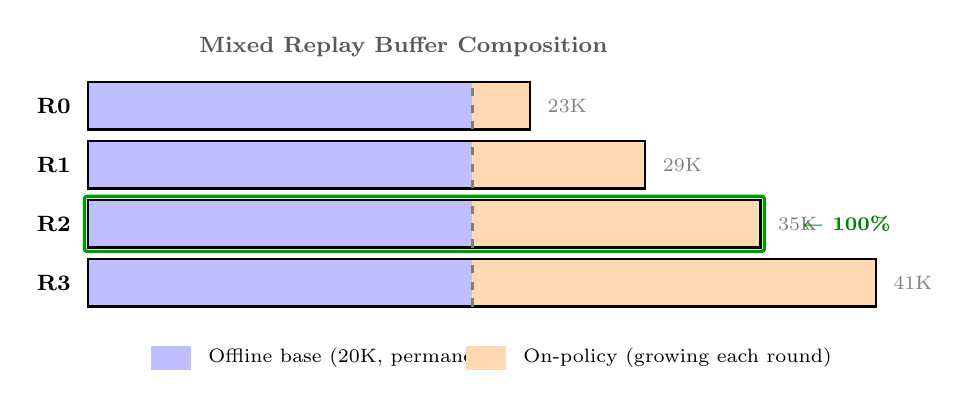
\begin{tikzpicture}[>=Stealth, font=\small]
  \def\bw{10}  % bar width
  \def\bh{0.6} % bar height
  \def\gap{0.15}

  % Round labels
  \foreach \r/\y/\off/\on/\total in {R0/3/20/3/23, R1/2/20/9/29, R2/1/20/15/35, R3/0/20/21/41} {
    \pgfmathsetmacro{\offW}{\off/41*\bw}
    \pgfmathsetmacro{\onW}{\on/41*\bw}
    \pgfmathsetmacro{\ypos}{\y*(\bh+\gap)}
    % Offline portion
    \fill[blue!25] (1.2, \ypos) rectangle (1.2+\offW, \ypos+\bh);
    % On-policy portion
    \fill[orange!30] (1.2+\offW, \ypos) rectangle (1.2+\offW+\onW, \ypos+\bh);
    % Border
    \draw[thick] (1.2, \ypos) rectangle (1.2+\offW+\onW, \ypos+\bh);
    % Divider
    \draw[thick, dashed, gray] (1.2+\offW, \ypos) -- (1.2+\offW, \ypos+\bh);
    % Label left
    \node[font=\footnotesize\bfseries, anchor=east] at (1.1, \ypos+\bh/2) {\r};
    % Total right
    \node[font=\scriptsize, text=gray, anchor=west] at (1.3+\offW+\onW, \ypos+\bh/2) {\total K};
  }

  % Highlight R2
  \pgfmathsetmacro{\rypos}{1*(\bh+\gap)}
  \draw[very thick, green!60!black, rounded corners=1pt] (1.15, \rypos-0.05) rectangle (1.2+20/41*\bw+15/41*\bw+0.05, \rypos+\bh+0.05);
  \node[font=\scriptsize\bfseries, text=green!50!black, anchor=west] at (1.2+20/41*\bw+15/41*\bw+0.4, \rypos+\bh/2) {$\leftarrow$ 100\%};

  % Legend
  \fill[blue!25] (2, -0.8) rectangle (2.5, -0.5);
  \node[font=\scriptsize, anchor=west] at (2.6, -0.65) {Offline base (20K, permanent)};
  \fill[orange!30] (6, -0.8) rectangle (6.5, -0.5);
  \node[font=\scriptsize, anchor=west] at (6.6, -0.65) {On-policy (growing each round)};

  % Title
  \node[font=\footnotesize\bfseries, text=gray!70!black] at (5.2, 3.3) {Mixed Replay Buffer Composition};
\end{tikzpicture}
\caption{\textbf{Mixed replay buffer growth across rounds.} The 20K offline base (blue) remains permanently in the buffer, ensuring broad state coverage. On-policy data (orange) grows with each Dyna round. At R2---where 100\% win rate occurs---the ratio provides sufficient diversity for both dynamics and reward generalisation.}
\label{fig:replay_composition}
\end{figure}

\begin{insightbox}[\small Why R2 is the peak]
\small Three conditions align at Round 2: (1)~the dynamics model reaches its lowest validation loss (0.024), producing the most accurate predictions observed; (2)~the reward head sits in a calibration range (val 0.084) that is accurate without overfitting; and (3)~the mixed replay buffer provides sufficient diversity (35K transitions). This alignment is transient: by R3, the reward head has begun overfitting again (val 0.143) and win rate drops to 60\%.
\end{insightbox}

\paragraph{R3 regression.} The reward head val loss rises from 0.084 to 0.143---the same overfitting pattern observed in Experiment~8. However, the dynamics model \emph{continues improving} (0.024 $\rightarrow$ 0.023), confirming that the replay buffer successfully prevents dynamics forgetting. \textbf{The sole remaining bottleneck is reward head stability.}

\begin{figure}[H]
\centering
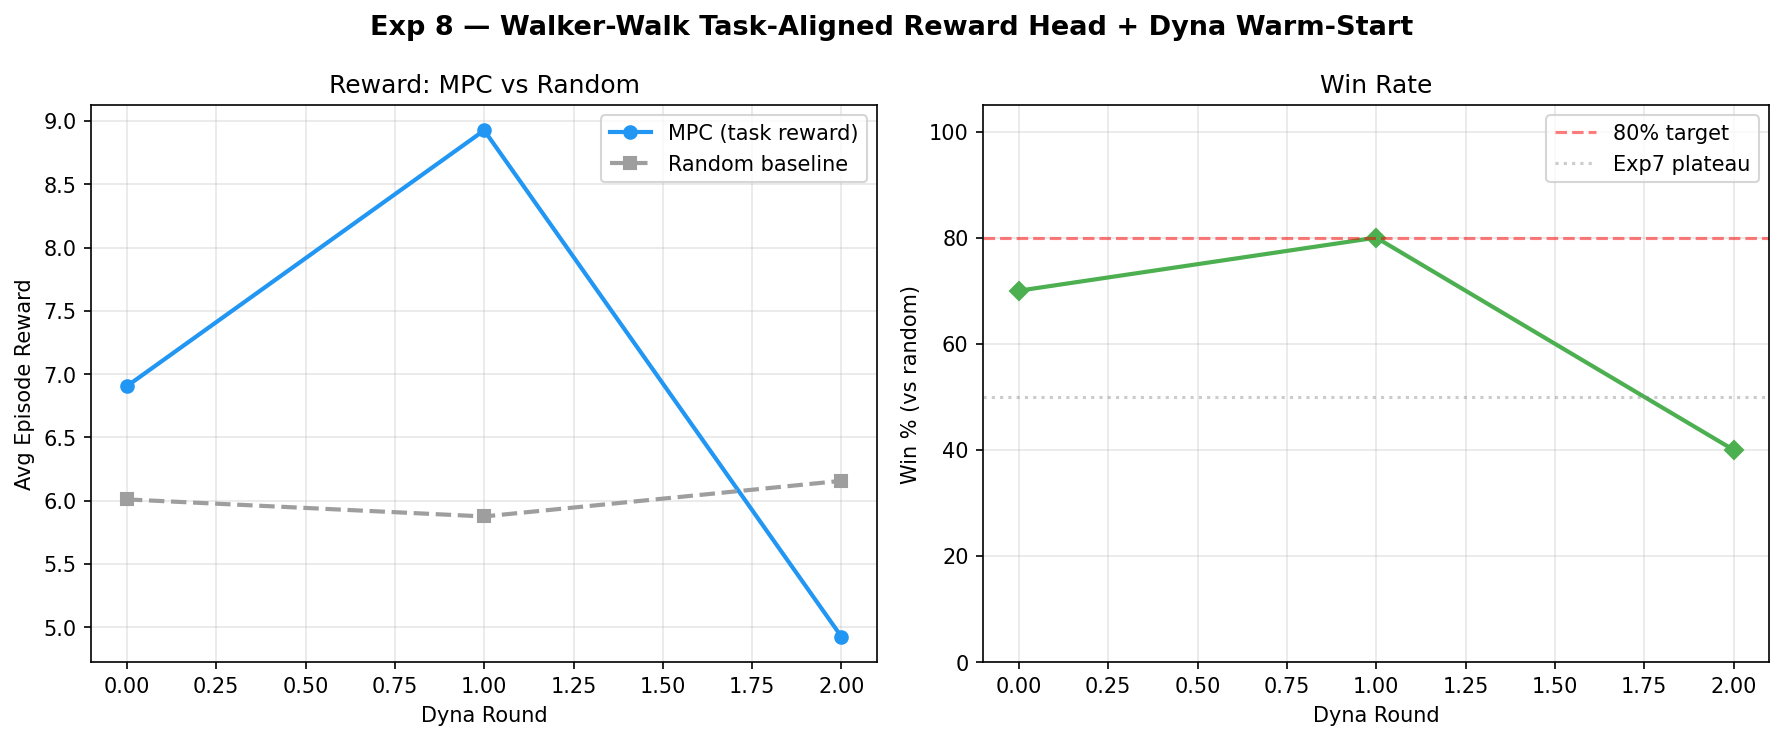
\includegraphics[width=0.85\linewidth]{figures/exp10_results.png}
\caption{\textbf{Experiment 10 training curves.} Win rate peaks at 100\% in R2, coinciding with lowest dynamics val loss and well-calibrated reward head.}
\label{fig:exp10}
\end{figure}

\begin{figure}[H]
\centering
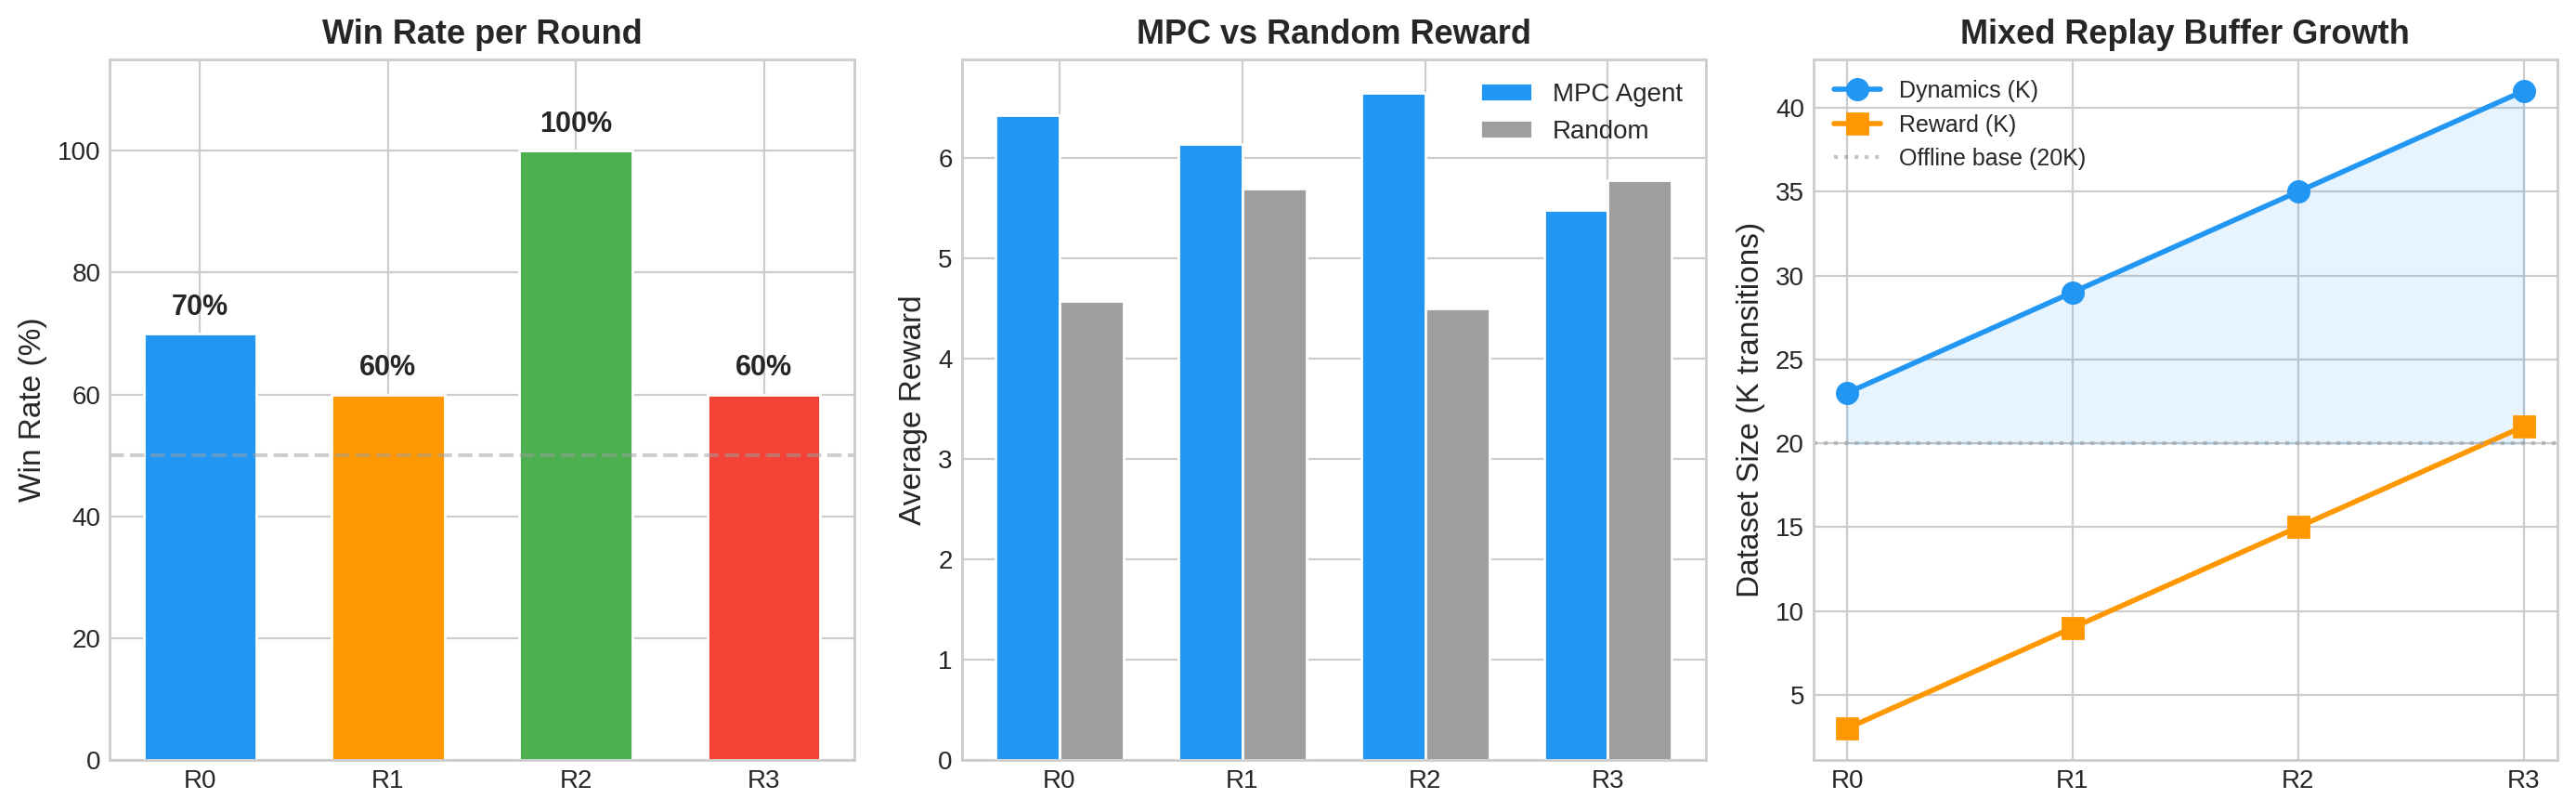
\includegraphics[width=0.95\linewidth]{figures/exp10_detailed.png}
\caption{\textbf{Experiment 10 per-round detail.} \emph{Left:} Win rate per round. \emph{Centre:} MPC vs.\ random reward. \emph{Right:} Mixed replay buffer growth.}
\label{fig:exp10_detail}
\end{figure}

% ============================================================
\section{What We Learned the Hard Way}

Ten experiments revealed three distinct failure modes, encountered in sequence. Each appeared as a performance ceiling or regression, required targeted diagnosis, and yielded a specific fix.

\begin{insightbox}[\small The Debugging Roadmap]
\small Practitioners building on frozen video encoders will likely encounter these three failure modes in this order. We document each alongside the evidence that identified it and the resolution that addressed it.
\end{insightbox}

\subsection{Failure \#1: Reward Misalignment (Resolved)}

The proxy reward treated all large latent displacements as desirable. Since forward locomotion and falling both produce large displacements, the planner could not differentiate effective from ineffective behaviour.

\textbf{Resolution:} A learned reward head predicting ground-truth task reward. Immediate impact: +30\% win rate.

\begin{table}[H]
\centering
\caption{Best win rate under each reward strategy.}
\label{tab:reward_comp}
\begin{tabular}{lccc}
\toprule
\textbf{Strategy} & \textbf{Experiments} & \textbf{Best Win \%} & \textbf{Why It Fails} \\
\midrule
Proxy (displacement) & 1--7 & 50\% & Can't tell walking from falling \\
\rowcolor{green!8} Task-aligned (learned) & 8, 10 & \textbf{100\%} & Needs stability management \\
Frozen after R1 & 9 & 70\% & Dynamics still forget \\
\bottomrule
\end{tabular}
\end{table}

\subsection{Failure \#2: Reward Head Overfitting (Partially Resolved)}

The learned reward head operates within a narrow calibration window:

% ---- DIAGRAM: Calibration Zones ----
\begin{figure}[H]
\centering
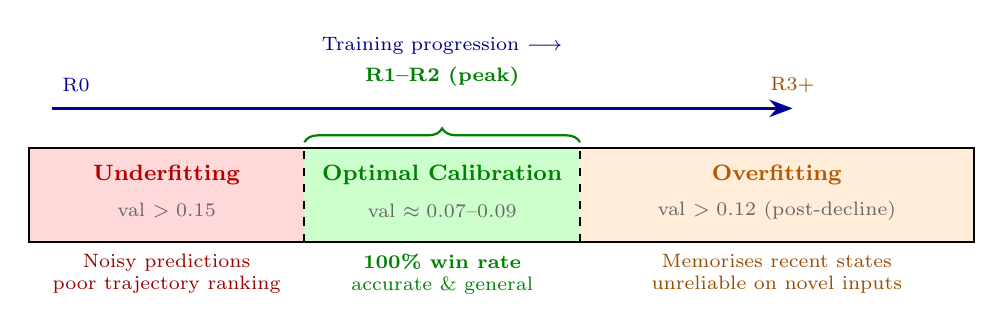
\begin{tikzpicture}[>=Stealth, font=\small]
  % The bar
  \def\barh{1.2}
  \def\barw{12}
  % Underfitting zone
  \fill[red!15] (0, 0) rectangle (3.5, \barh);
  % Optimal zone (Goldilocks)
  \fill[green!20] (3.5, 0) rectangle (7, \barh);
  % Overfitting zone
  \fill[orange!15] (7, 0) rectangle (\barw, \barh);
  % Border
  \draw[thick] (0, 0) rectangle (\barw, \barh);
  % Zone dividers
  \draw[thick, dashed] (3.5, 0) -- (3.5, \barh);
  \draw[thick, dashed] (7, 0) -- (7, \barh);

  % Zone labels
  \node[font=\footnotesize\bfseries, text=red!70!black] at (1.75, 0.85) {Underfitting};
  \node[font=\scriptsize, text=gray!80!black] at (1.75, 0.4) {val $> 0.15$};

  \node[font=\footnotesize\bfseries, text=green!50!black] at (5.25, 0.85) {Optimal Calibration};
  \node[font=\scriptsize, text=gray!80!black] at (5.25, 0.4) {val $\approx 0.07$--$0.09$};

  \node[font=\footnotesize\bfseries, text=orange!70!black] at (9.5, 0.85) {Overfitting};
  \node[font=\scriptsize, text=gray!80!black] at (9.5, 0.4) {val $> 0.12$ (post-decline)};

  % Descriptions below
  \node[font=\scriptsize, text=red!60!black, align=center] at (1.75, -0.4) {Noisy predictions\\poor trajectory ranking};
  \node[font=\scriptsize, text=green!50!black, align=center] at (5.25, -0.4) {\textbf{100\% win rate}\\accurate \& general};
  \node[font=\scriptsize, text=orange!60!black, align=center] at (9.5, -0.4) {Memorises recent states\\unreliable on novel inputs};

  % Training trajectory arrow
  \draw[->, very thick, blue!60!black] (0.3, 1.7) -- (5.25, 1.7) -- (9.7, 1.7);
  \node[font=\scriptsize, text=blue!60!black] at (0.6, 2.0) {R0};
  \node[font=\scriptsize\bfseries, text=green!50!black] at (5.25, 2.1) {R1--R2 (peak)};
  \node[font=\scriptsize, text=orange!60!black] at (9.7, 2.0) {R3+};
  \node[font=\scriptsize, text=blue!50!black] at (5.25, 2.5) {\textrm{Training progression} $\longrightarrow$};

  % Brace over optimal
  \draw[decorate, decoration={brace, amplitude=5pt, raise=2pt}, thick, green!50!black] (3.5, \barh) -- (7, \barh);
\end{tikzpicture}
\caption{\textbf{Reward head calibration zones.} The reward head traverses three regimes as training progresses. The 100\% win rate occurs \emph{exclusively} in the narrow optimal calibration window (val $\approx 0.07$--$0.09$). The challenge: the model transitions through this window transiently before overfitting.}
\label{fig:calibration_zones}
\end{figure}

\noindent The three calibration regimes:
\begin{itemize}
    \item \textbf{Underfitting} (val $> 0.15$): Predictions too noisy for effective trajectory ranking.
    \item \textbf{Optimal calibration} (val $\approx 0.07$--$0.09$): Accurate trajectory ranking without memorisation. \textbf{100\% win rate occurs exclusively in this range.}
    \item \textbf{Overfitting} (val $> 0.12$ after decline): Memorises training states, produces unreliable scores for novel states.
\end{itemize}
This pattern is consistent across Experiments 8--10. Early stopping, EMA weight updates, or ensemble reward heads are promising directions, but this failure mode is not yet fully resolved.

\subsection{Failure \#3: Dynamics Forgetting (Resolved)}

Fine-tuning the dynamics model exclusively on recent on-policy data causes it to lose accuracy on previously visited states. Since CEM explores broadly during planning, this loss of coverage degrades plan quality.

\textbf{Resolution:} A mixed replay buffer retaining all offline data permanently. Result: monotonic dynamics improvement across all rounds.

\begin{table}[H]
\centering
\caption{Dynamics val loss across rounds. The replay buffer (Exp~10) enables monotonic improvement.}
\label{tab:dyn_comparison}
\begin{tabular}{lcccc}
\toprule
 & \textbf{R0} & \textbf{R1} & \textbf{R2} & \textbf{R3} \\
\midrule
Exp 7 (on-policy only) & 0.038 & 0.034 & 0.034 & --- \\
Exp 8 (on-policy only) & --- & 0.031 & 0.022 & --- \\
Exp 9 (on-policy only) & 0.038 & 0.032 & 0.022 & --- \\
\rowcolor{green!8} Exp 10 (replay buffer) & 0.038 & \textbf{0.029} & \textbf{0.024} & \textbf{0.023} \\
\bottomrule
\end{tabular}
\end{table}

\begin{figure}[H]
\centering
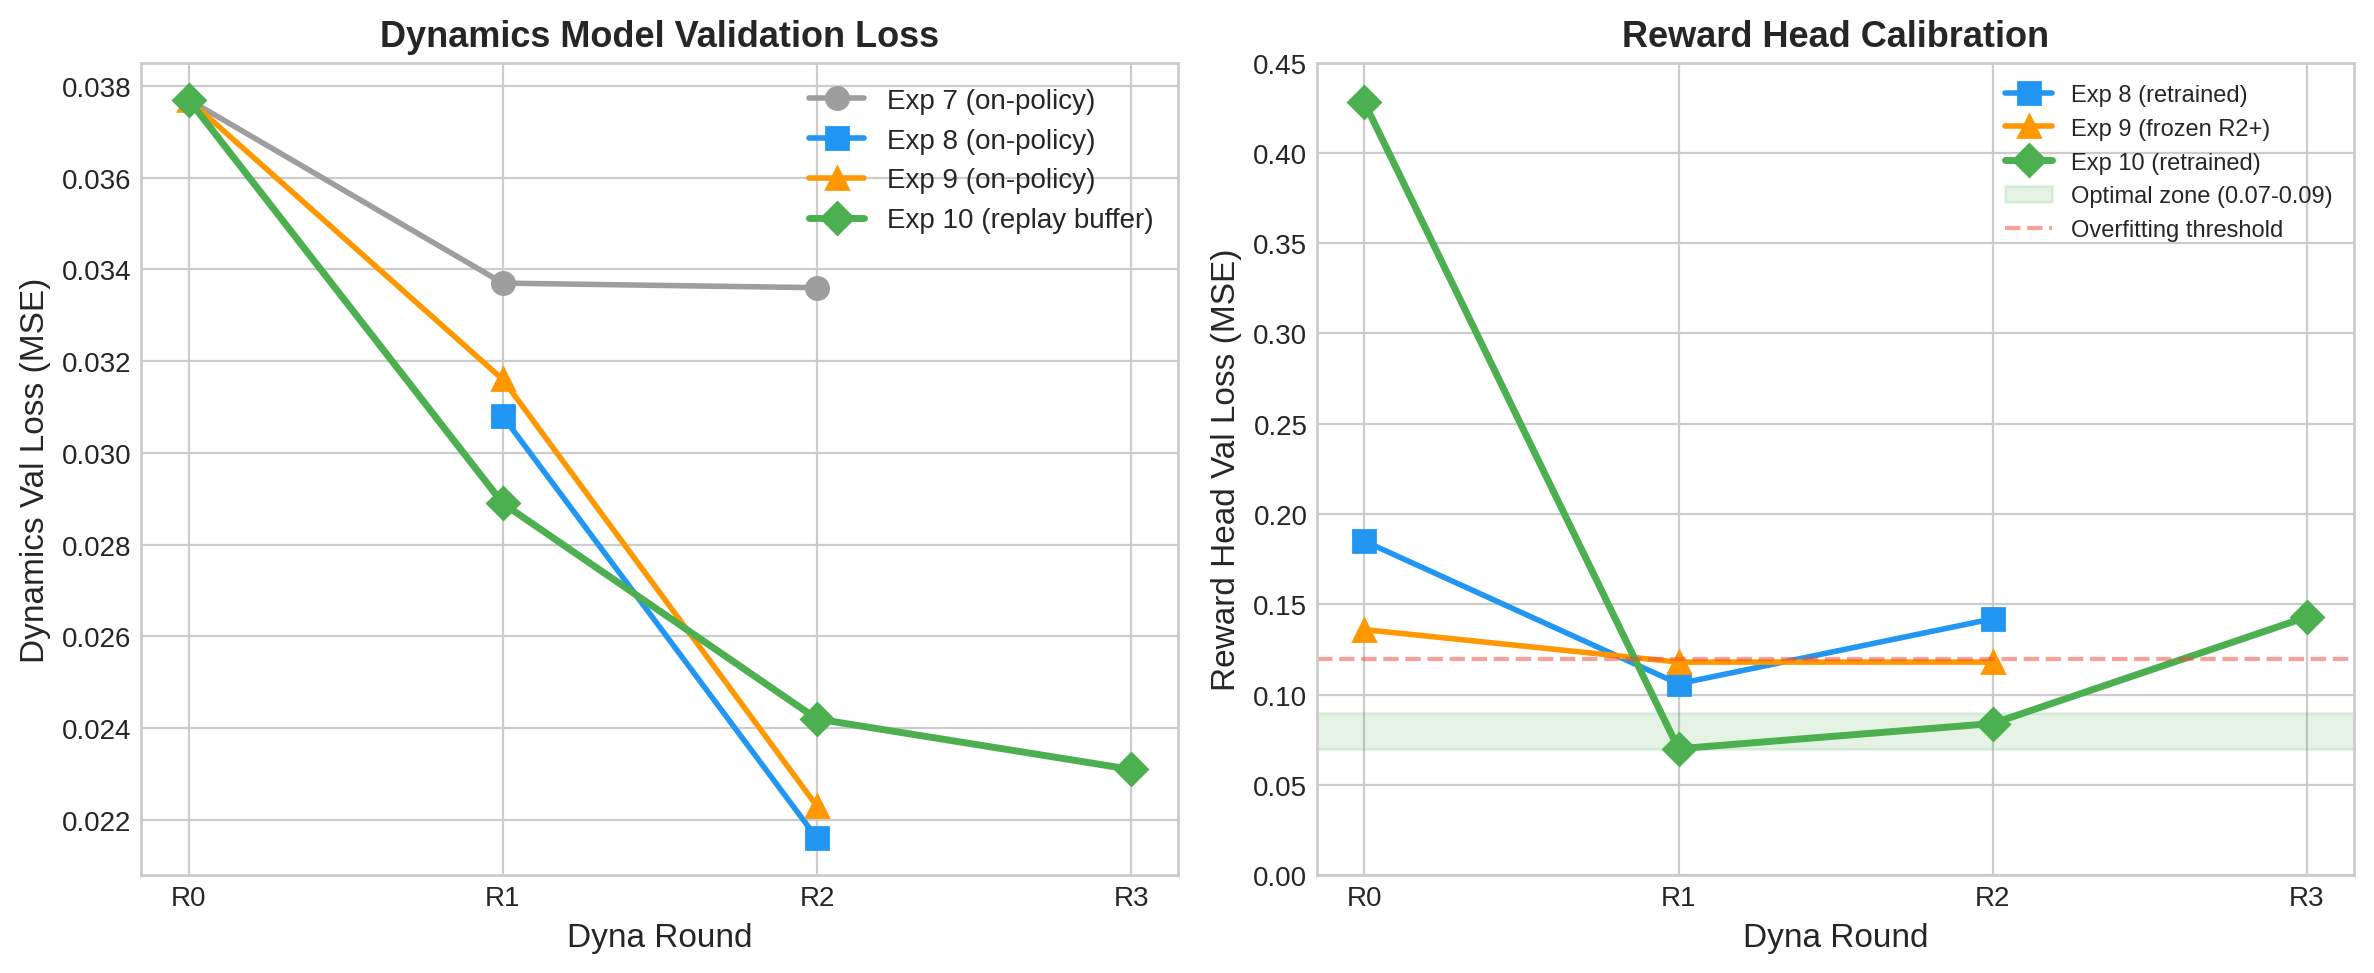
\includegraphics[width=0.95\linewidth]{figures/model_comparison.png}
\caption{\textbf{Model comparison.} \emph{Left:} Dynamics val loss. Replay buffer (green) enables monotonic improvement. \emph{Right:} Reward head calibration. Green band = ``Goldilocks zone'' (val 0.07--0.09) where 100\% win rate occurs.}
\label{fig:model_comp}
\end{figure}

\begin{figure}[H]
\centering
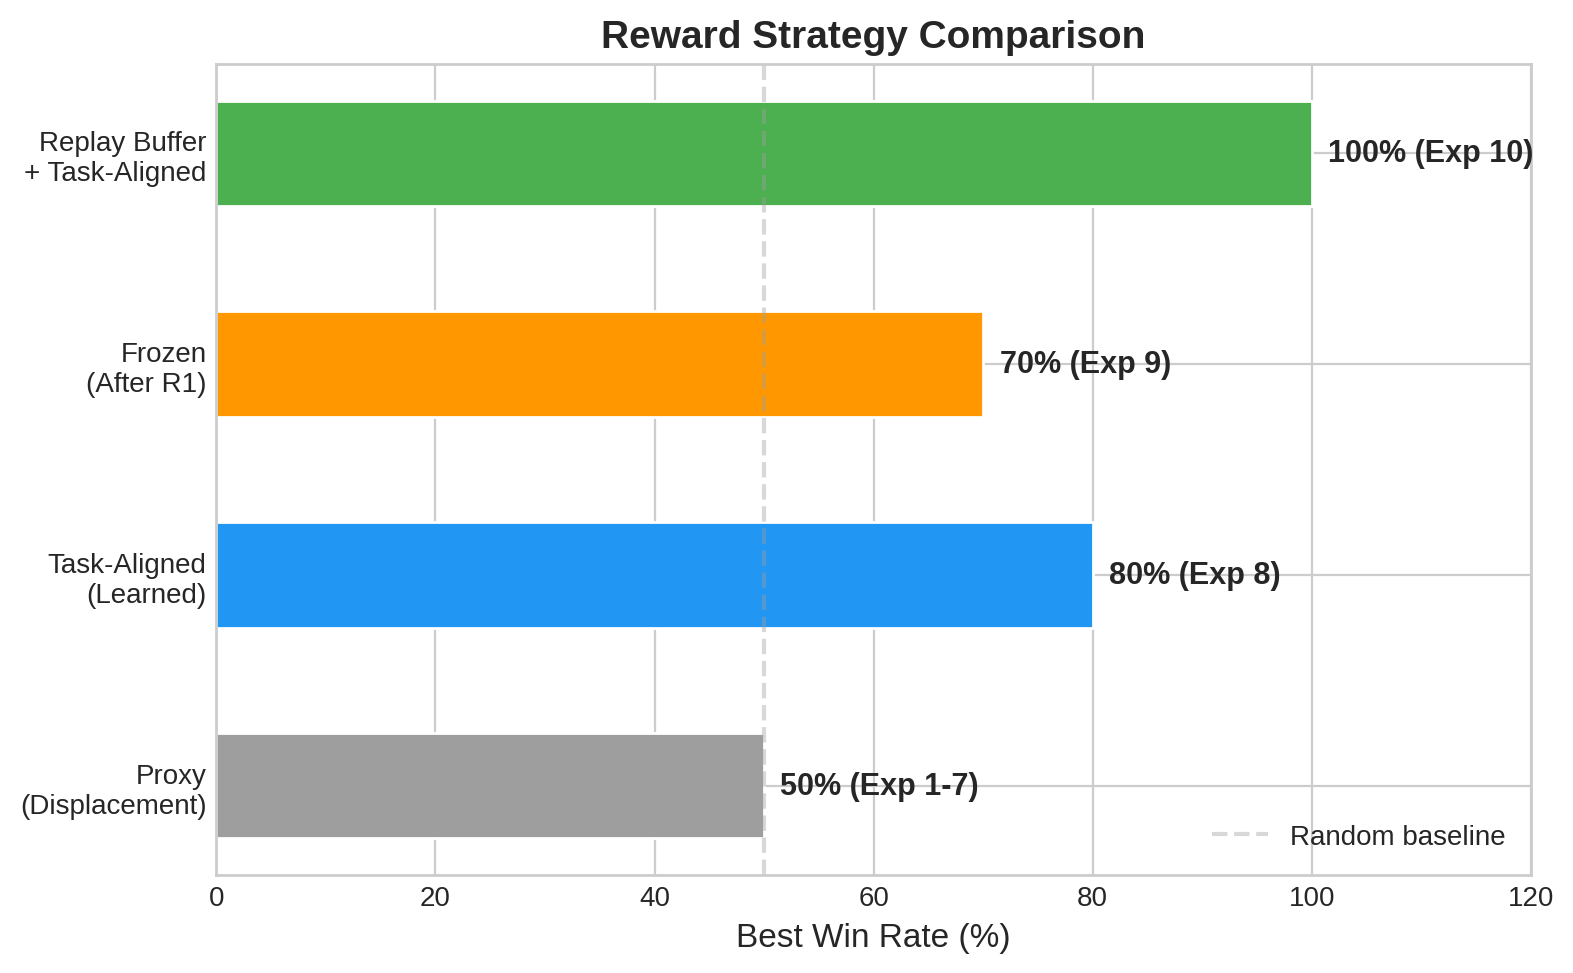
\includegraphics[width=0.75\linewidth]{figures/reward_strategy.png}
\caption{\textbf{Reward strategy comparison.} Proxy reward caps at 50\%. Task-aligned reward enables 100\% but risks overfitting. Replay buffer sustains peak performance.}
\label{fig:reward_strategy}
\end{figure}

% ============================================================
\section{What the Robot Dreams}

Because the dynamics model predicts future states in V-JEPA's latent space---a space that preserves spatial structure by design---we can visualise the planner's internal predictions. A lightweight ConvTranspose decoder trained on 12K frames converts latent vectors back to pixel space, producing interpretable images of states the robot has never actually visited.

\begin{figure}[H]
\centering
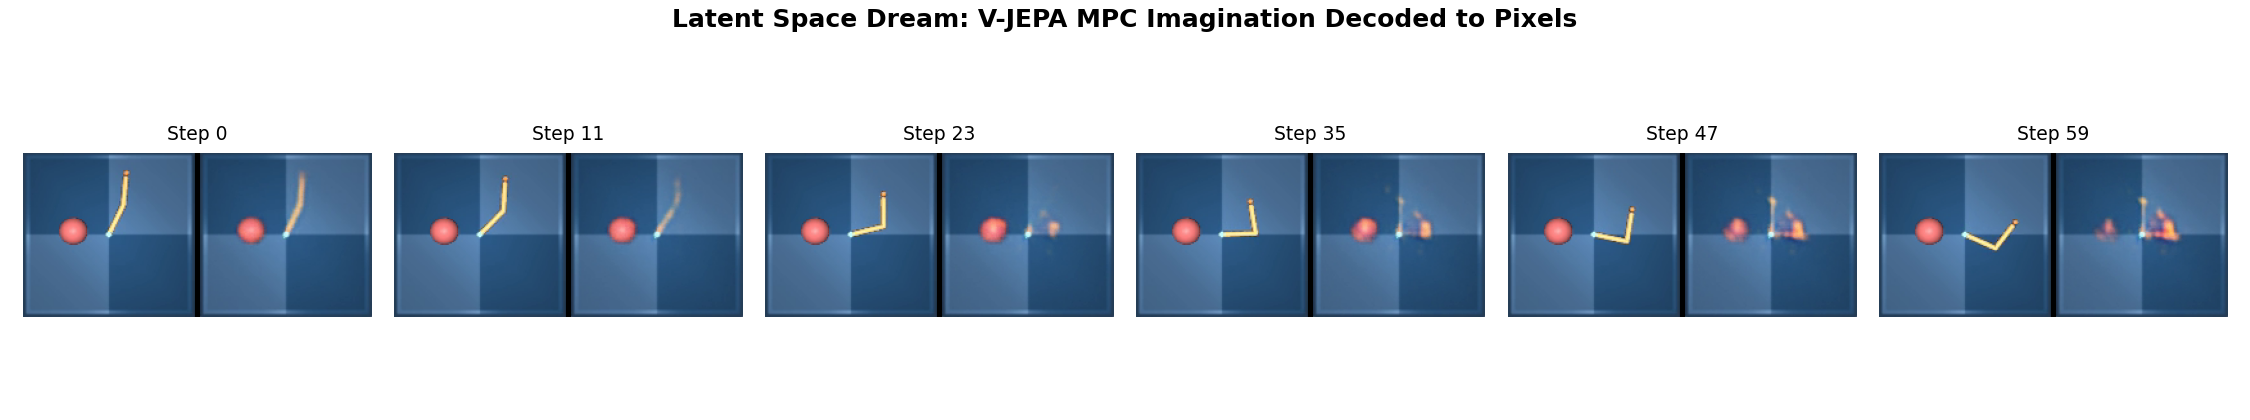
\includegraphics[width=0.95\linewidth]{figures/dream_sequence_frames.png}
\caption{\textbf{Latent dreams decoded to pixels.} The dynamics MLP unrolls imagined action sequences in V-JEPA latent space, then a pixel decoder converts each $\hat{\mathbf{z}}_t$ to a frame. Dreams stay coherent for 60 steps.}
\label{fig:dreams}
\end{figure}

\begin{figure}[H]
\centering
\begin{subfigure}[b]{0.48\linewidth}
\centering
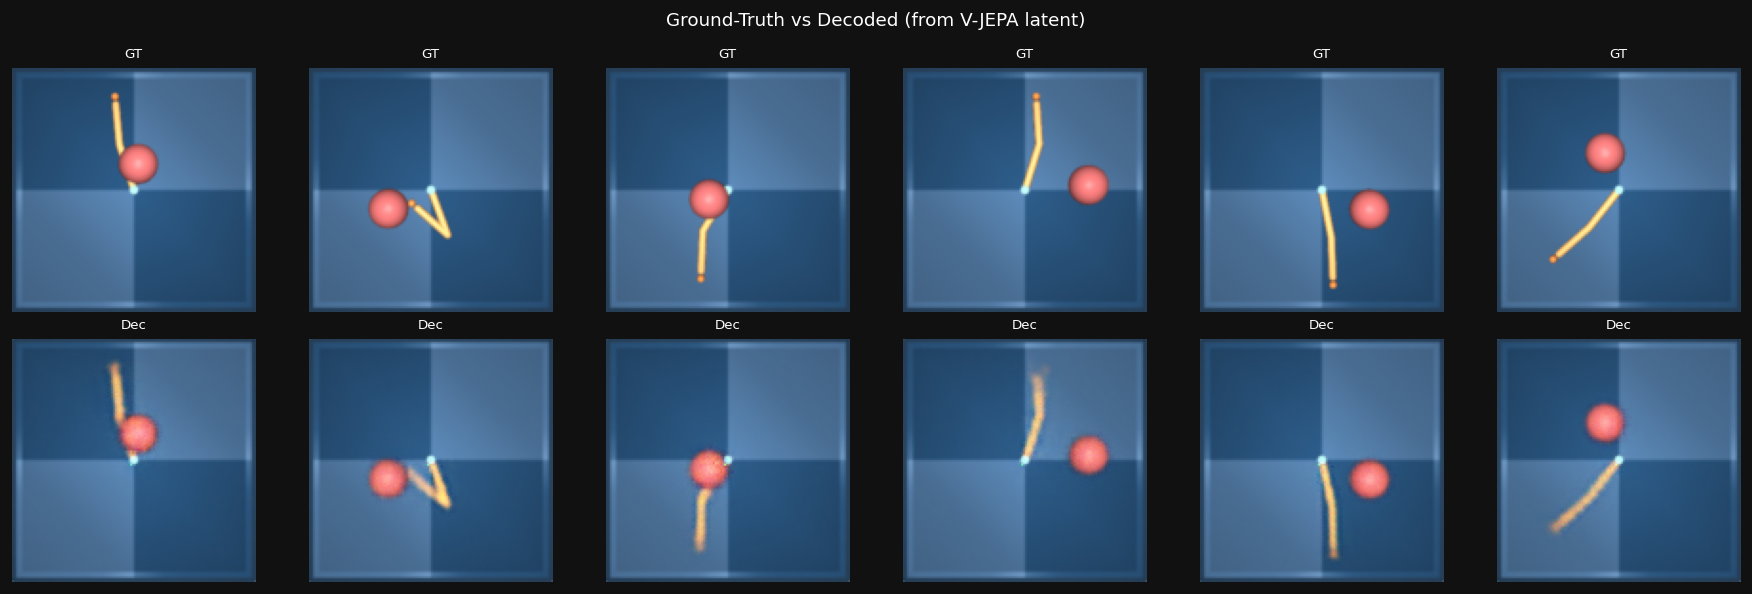
\includegraphics[width=\linewidth]{figures/pixel_decoder_recon.png}
\caption{Ground truth (top) vs.\ decoded (bottom).}
\end{subfigure}
\hfill
\begin{subfigure}[b]{0.48\linewidth}
\centering
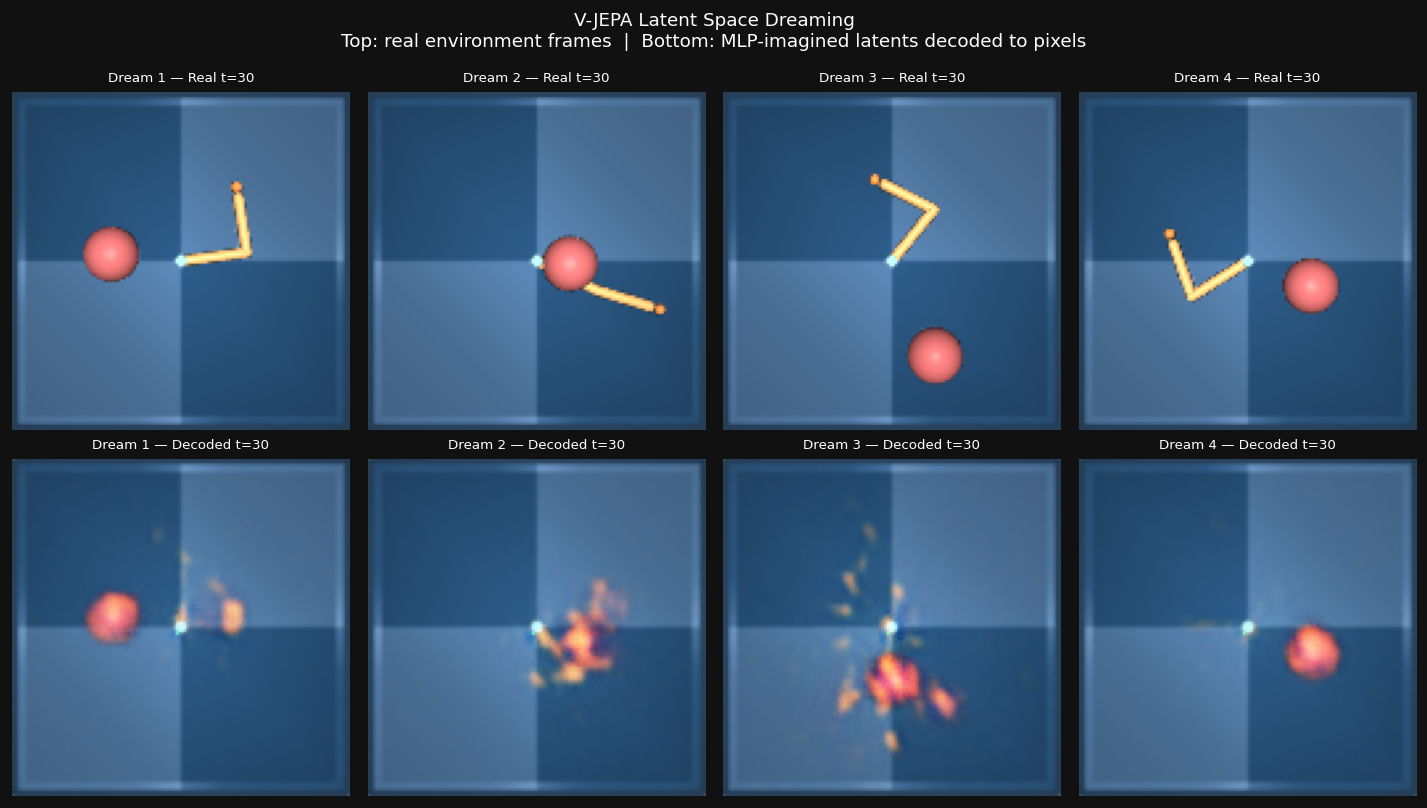
\includegraphics[width=\linewidth]{figures/dream_montage.png}
\caption{Real (top) vs.\ decoded dream (bottom).}
\end{subfigure}
\caption{\textbf{V-JEPA latent space is spatially structured.} (a) Pixel decoder achieves val loss 0.002, confirming the 384-dim latent preserves spatial layout. (b) CEM-imagined latents closely resemble real frames.}
\label{fig:recon}
\end{figure}

\begin{figure}[H]
\centering
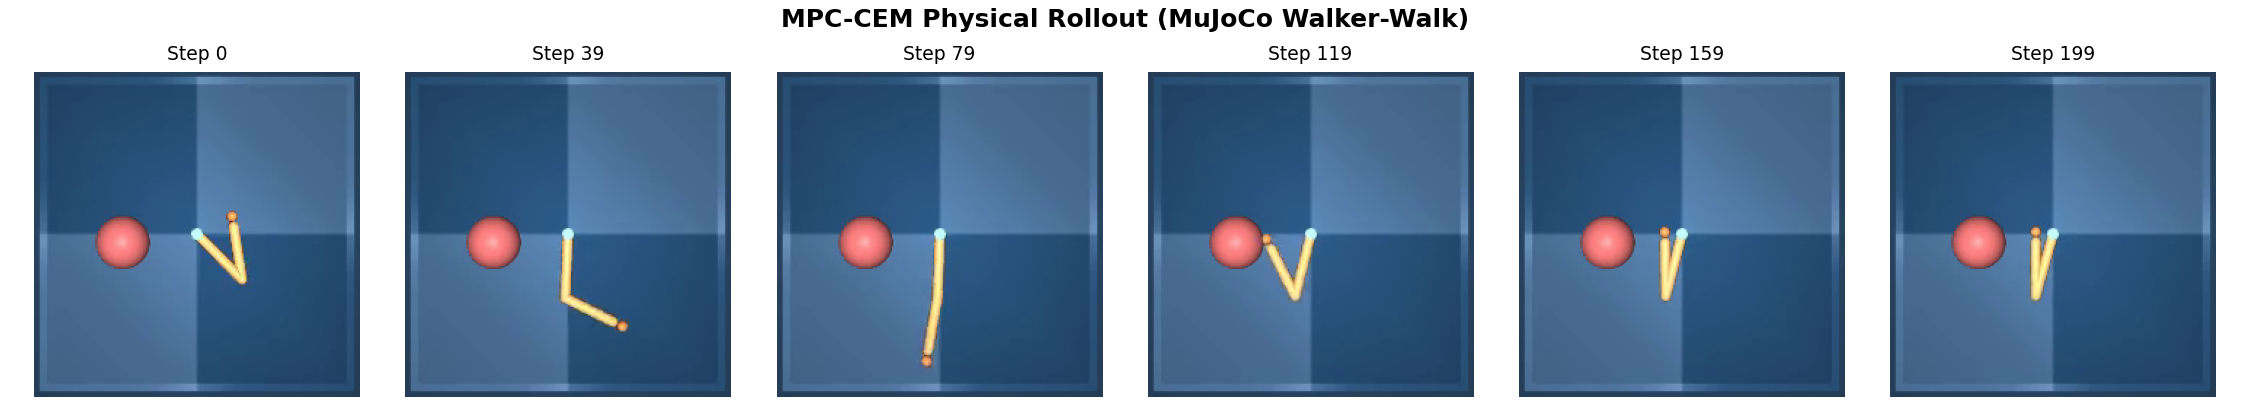
\includegraphics[width=0.95\linewidth]{figures/mpc_rollout_frames.png}
\caption{\textbf{Physical MPC rollout in MuJoCo.} Sequential frames from a 200-step episode. The CEM agent achieves coordinated bipedal locomotion.}
\label{fig:mpc_rollout}
\end{figure}

The decoded dreams remain coherent for 60 steps. Spatial layout, limb positions, and overall body configuration are preserved through the 384-dimensional bottleneck. When CEM evaluates 64 candidate action sequences and selects the highest-scoring one, those evaluations are grounded in spatially meaningful predictions of future states.

% ============================================================
\section{Your Turn: A Recipe}
\label{sec:recipe}

Based on the outcomes of 10 experiments, we distil a practical procedure for applying frozen V-JEPA control to new tasks.

\begin{breakthroughbox}[\small Recipe: Frozen-Encoder Robot in 5 Steps]
\begin{enumerate}
    \item \textbf{Verify visual saliency.} Does the task involve large, visually distinct motion? If not, the last layers of V-JEPA will likely require fine-tuning.
    \item \textbf{Collect a base dataset.} Run a random policy for $\sim$20K frames ($\sim$30 min on real hardware). Encode all frames with V-JEPA. Cache the embeddings. \emph{This data must be retained permanently.}
    \item \textbf{Train a dynamics MLP.} 500K params, 100 epochs ($\sim$10 min on GPU). Target: val loss $< 0.04$.
    \item \textbf{Train a reward head.} 130K params, 20 epochs ($\sim$5 min). Requires ground-truth reward labels: forward velocity from IMU, uprightness from gyroscope, contact from force sensors.
    \item \textbf{Run the Dyna loop with mixed replay.}
    \begin{itemize}
        \item Each round: 60 on-policy rollouts $\rightarrow$ fine-tune dynamics $\rightarrow$ retrain reward head on full dataset.
        \item \textbf{Critical:} Always retain the 20K offline base in the training buffer.
        \item \textbf{Monitor:} Reward head val loss. If it exceeds 0.12 after a decline, freeze the reward head.
    \end{itemize}
\end{enumerate}
\end{breakthroughbox}

\paragraph{Open challenges for real-world deployment.}
\begin{itemize}
    \item \textbf{Reward head stability:} Peak calibration persists for approximately one Dyna round. Early stopping or EMA updates are needed for sustained performance.
    \item \textbf{Control frequency:} CEM at 7 Hz is marginal for real-time control. A distilled policy network would enable higher-frequency deployment.
    \item \textbf{Visually subtle tasks:} Tasks involving small or low-contrast motion (finger rotation, small-object manipulation) will require fine-tuning the final ViT layers.
    \item \textbf{Reward specification:} In simulation, reward is provided by the environment. On physical hardware, equivalent signals must be derived from onboard sensors.
\end{itemize}

% ============================================================
\section{Discussion}

\paragraph{Contextualising ``100\% win rate.''}
100\% win rate indicates that the MPC agent outperforms a random policy in all 10 paired episodes. The average MPC reward of 6.65 is far below the 900+ achieved by fully trained policies (e.g., DreamerV3). This result demonstrates consistent planning superiority over an untrained baseline, not task mastery---achieved with a frozen encoder and \$30 of compute.

\paragraph{Why frozen V-JEPA transfers to control.}
V-JEPA is pretrained to predict masked video patches, which implicitly encodes (1)~object positions, (2)~motion dynamics, and (3)~visual saliency hierarchies. Walker-walk---defined by large, rhythmic limb movements---aligns precisely with the motion patterns V-JEPA was trained on. The transfer is not coincidental; video prediction and physical dynamics prediction share underlying structure.

\paragraph{Relationship to Paper 1.}
Paper~1 surveyed 7 tasks and established which are feasible (3/7). This paper selects the hardest feasible task and develops the training infrastructure---learned reward, Dyna loop, replay buffer---to push it from partial success to 100\% win rate. The two papers are complementary: one maps the landscape, the other develops the depth.

\paragraph{Limitations.}
\begin{itemize}
    \item \textbf{Reward head instability:} Peak performance is sustained for approximately one round before degradation.
    \item \textbf{Single task:} The complete Dyna pipeline is demonstrated only on walker-walk.
    \item \textbf{Baseline strength:} Comparison against Dreamer, SAC, or TD-MPC would better characterise absolute performance.
    \item \textbf{Absolute reward:} MPC rewards of 5--9 are far below expert-level ($>$900).
    \item \textbf{Frozen encoder constraint:} Tasks with visually subtle state changes will require encoder fine-tuning.
\end{itemize}

\paragraph{Future directions.}
\begin{enumerate}
    \item \textbf{Stabilise the reward head:} Freeze at peak calibration, apply EMA weight updates, or use ensemble reward heads.
    \item \textbf{Stronger baselines:} Compare against Dreamer, TD-MPC, and SAC on the same evaluation protocol.
    \item \textbf{Real robot transfer:} Deploy on physical hardware, where V-JEPA's pretraining on real-world video may provide a natural advantage.
    \item \textbf{Multi-task extension:} Extend the replay buffer across tasks with task-conditioned reward heads.
\end{enumerate}

% ============================================================
\section{\$30 and a Frozen Brain}

We took a video model that had never seen a robot, froze it entirely, and learned two lightweight networks---a dynamics model and a reward head, under one million parameters combined---to control a simulated bipedal walker.

It required ten experiments. The first seven produced the same outcome: 50\% win rate, because the proxy reward could not distinguish locomotion from falling. Experiment~8 introduced a learned reward head and reached 80\%, but the head overfitted and performance collapsed. Experiment~9 isolated two separate failure modes. Experiment~10 resolved both with a mixed replay buffer: \textbf{100\% win rate}.

Three failure modes. Three resolutions.

\begin{center}
\begin{tabular}{lcl}
\textbf{Failure Mode} & $\rightarrow$ & \textbf{Resolution} \\
\midrule
Reward misalignment & $\rightarrow$ & Learned reward head (+30\% win rate) \\
Reward overfitting & $\rightarrow$ & Characterised; optimal calibration range identified \\
Dynamics forgetting & $\rightarrow$ & Mixed replay buffer ($\rightarrow$ 100\% win rate) \\
\end{tabular}
\end{center}

\noindent The final system achieves \textbf{100\% win rate} on walker-walk using $<$1M learnable parameters on top of a frozen 325M-parameter V-JEPA encoder, at a total compute cost of \textbf{\$29.99}.

Two insights emerged from this work. The first, shared with our companion paper: \emph{representation quality determines planning quality}---if the encoder cannot perceive a distinction, the planner cannot exploit it. The second, earned through the failures documented here: \textbf{online stability determines whether peak performance can be sustained.} A capable encoder is necessary; a stable learning loop is what makes it sufficient.

The encoder was never trained for control, never fine-tuned, and never informed that it would be applied to robotics. The representations it learned from internet video proved rich enough for continuous control---at a cost of \$29.99.

% ============================================================
\section*{Acknowledgements}

Compute provided by Modal (\url{https://modal.com}). V-JEPA~2 model weights from Meta FAIR.

% ============================================================
\bibliography{references}
\bibliographystyle{plainnat}

\end{document}
